\documentclass[../Main.tex]{subfiles}

\begin{document}
\author{Wave Graphs} %use author for title of lesson
\date{Year 1 Topic 16} %use date to refer to topic in main booklet

\section{Wave Graphs} %Section is the title of the lesson repeated, ready for the main contents page.

\begin{frame}{Displacement-distance graphs}
    A wave can be represented as a snapshot in time. In these we look at the profile of the wave. A displacement-distance graph can give us the wavelength and amplitude of the wave. 
    
    \begin{figure}
        \centering
        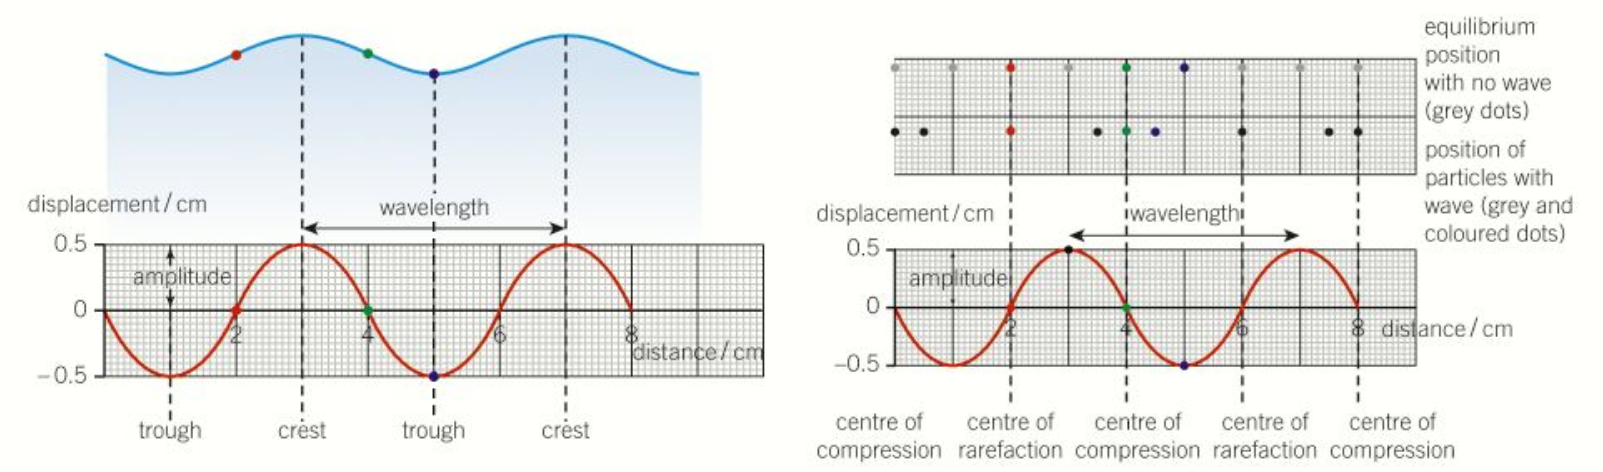
\includegraphics[width=\textwidth]{Waves_Images/displacement_distance_graph.png}
    \end{figure}
    
    This works for both transverse and longitudinal, although longitudinal waves are much harder to visualise.
\end{frame}

\begin{frame}{Displacement-distance graphs}
\begin{multicols}{2}
    If you want to see how a wave changes over time, you cannot do this with a single displacement-distance graph alone. 
    \newline \newline
    Instead, you can take multiple displacement-distance graphs at time intervals apart -- remember the particles themselves do not move, only the wave as a whole. 
        \newline \newline
    With these, each graph is $\frac{T}{4}$s apart, showing the perpendicular motion of a particle in a transverse wave.
    \columnbreak
    \begin{figure}
        \centering
        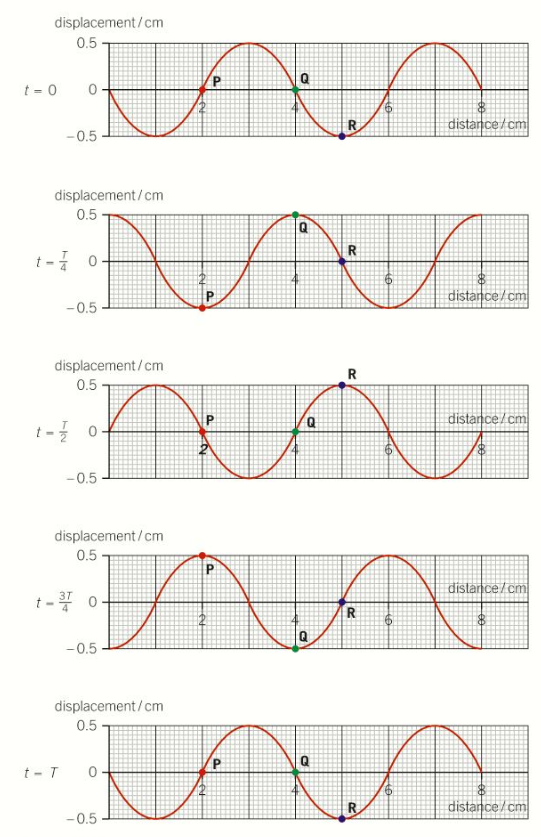
\includegraphics[height=7cm]{Waves_Images/displacement_distance_time_snapshots.png}
    \end{figure}
    \end{multicols}
\end{frame}
\begin{frame}{Units of Angle}
    Before we continue, we must first introduce a new unit of angle. 
    \begin{figure}
        \centering
        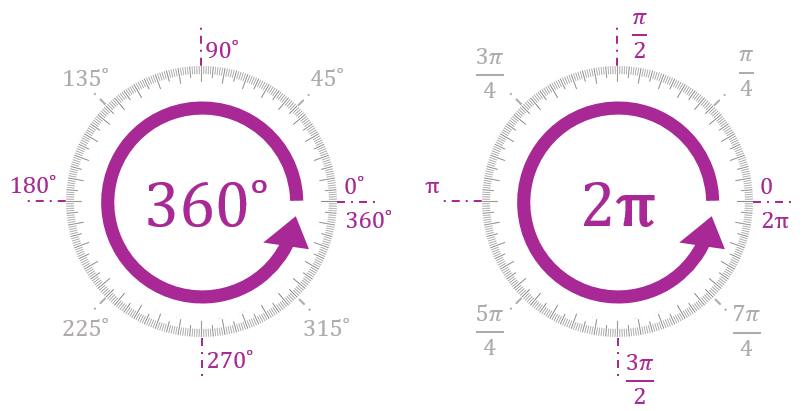
\includegraphics[height=4cm]{Waves_Images/radians.png}
    \end{figure}
    The radian is the natural unit of angle, defined by the radius and circumference of a circle. 1 radian is the angle subtended by an arc length equal to the radius of a circle. -- you do not need to know this definition!
    \newline \newline
    Some useful values to know are labelled.
\end{frame}

\begin{frame}{Radians vs Degrees}
\begin{itemize}
    \item There are $2\pi$ radians in a full rotation 
    \item 1 radian is approximately 57 degrees
\end{itemize}
\hspace{1cm}

To convert to radians from degrees, simply multiply by $\frac{\pi}{180}$. To convert from radians to degrees divide by $\frac{\pi}{180}$. 

\begin{exampleblock}{Example}
\begin{itemize}
    \item Convert 60 degrees to radians \pause
    -- $\frac{\pi}{3}$
    \item Convert $\frac{\pi}{4}$ radians to degrees \pause
    -- 45$^\circ$
\end{itemize}
\end{exampleblock}
\end{frame}

\begin{frame}{Phase Difference}
    Between any two points on a wave, we can say that they are in or out of phase. 
    
    \begin{itemize}
    \item If two points are in phase, it means that they are both at the same point at the same time, e.g at a peak, or trough, etc. 
    
    \item If two points are completely out of phase (antiphase), it means that they are at opposite points at the same time, e.g. one at a peak, and another at a trough
    \end{itemize}
\pause
\begin{figure}
    \centering
    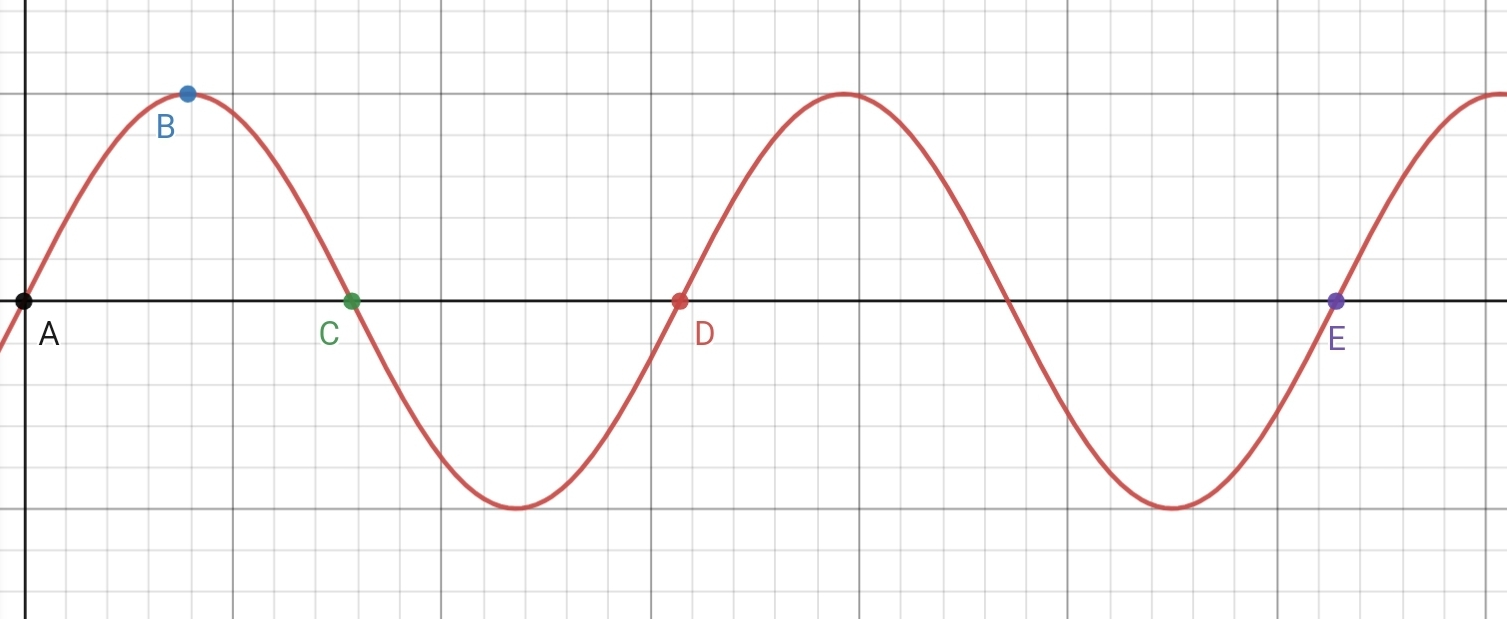
\includegraphics[height=2.5cm]{Waves_Images/wave_abcde.jpg}
\end{figure} \pause
In the above, the phase differences are as follows:
\begin{table}[]
\begin{tabular}{c|l|l|l|l|l}
\multirow{2}{*}{\begin{tabular}[c]{@{}c@{}}Phase Difference \\ from A\end{tabular}} & A & B & C & D & E \\ \cline{2-6} 
 & $0$ & $\frac{\pi}{2}$ & $\pi$ & $2\pi$ & $4\pi$
\end{tabular}%
\end{table}

\end{frame}

\begin{frame}{Phase Difference}
    Phase difference can be calculated.
    
    \begin{equation*}
        \phi = \frac{x}{\lambda} \times 2\pi 
    \end{equation*} (or $\times 360^\circ$ if in degrees)
    
    where: \begin{itemize}
        \item x = distance between two points -- units meters
        \item $\lambda$ = the wavelength -- units meters
        \item $2\pi$ or $360^\circ$ is the number of radians or degrees in a full cycle
    \end{itemize}
    \pause
    \begin{exampleblock}{Example}
    Two points on a wave are $\frac{\pi}{6}$ radians out of phase. The wavelength is 10 meters. Calculate the distance between the two points. \pause
    -- 0.83m
    \end{exampleblock}
\end{frame}

\begin{frame}{Displacement-time graphs}
    A displacement-time graph will track the motion of a single particle on a wave, plotting the displacement with time. 
    
    \begin{figure}
        \centering
        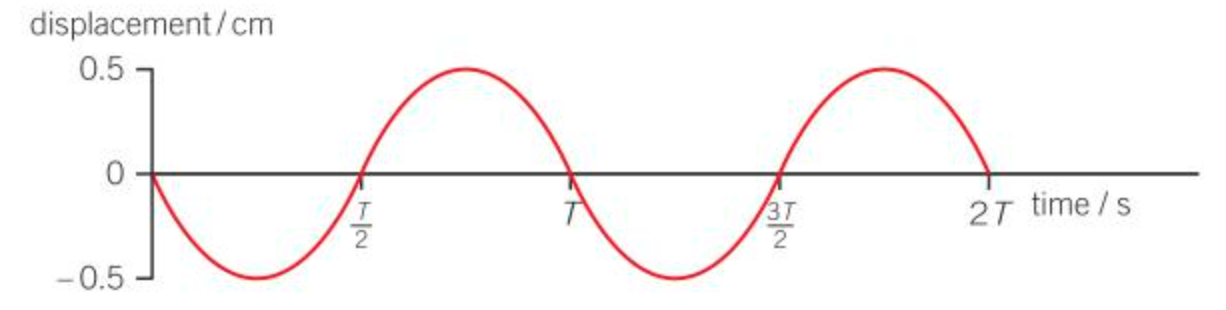
\includegraphics[width=\textwidth]{Waves_Images/displacement_time_graph.png}
    \end{figure}
    
    From it, we can find the time period (and hence frequency), and amplitude of a wave.
\end{frame}

\begin{frame}{S-d vs S-t graphs}
    \begin{figure}
        \centering
        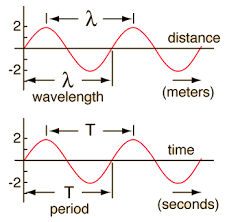
\includegraphics[height=4.5cm]{Waves_Images/sdst_comparison.png}
    \end{figure}
    The key difference is that a displacement-distance graph will give a wavelength, while a displacement-time graph will give a time period -- so check your axis!
\end{frame}

\begin{frame}{Example}
\begin{exampleblock}{}
    \begin{figure}
        \centering
        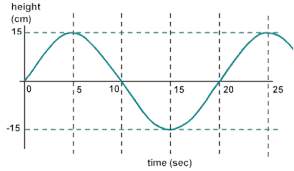
\includegraphics[height=4cm]{Waves_Images/example_wave_question.png}
    \end{figure}
    
    \begin{itemize}
        \item Determine the time period, and hence the frequency of this wave. \pause 
        -- T=20s, f=0.05Hz
        \item Given that this is a sound wave, calculate the wavelength \pause
        --$\lambda$=6600m
        \item Sketch a displacement-distance graph for this wave, labelling two points that are $\frac{\pi}{4}$ radians out of phase. \pause
        \item Calculate the distance between these two points. \pause
        --825m
    \end{itemize}
    \end{exampleblock} 
\end{frame}

\end{document}